\section{Treap}
\emph{Treap} stands for tree (as in binary search tree) + heap: every node is composed by a key and a priority (and of course the pointers to the children nodes, if any).
The key is used to make binary search tree while the priority is used for min/max heap.

Ex:
\begin{figure}[H]
    \centering
    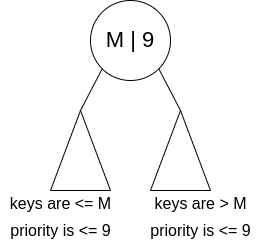
\includegraphics[width=150px]{images/4_Randomized_data_structures/treap_intro.png}
    \caption{Key are letters, priority is an integer, max heap}
\end{figure}

It's a data structure highly used in computational geometry, for example let's assume we have a bunch of points:
\begin{figure}[H]
    \centering
    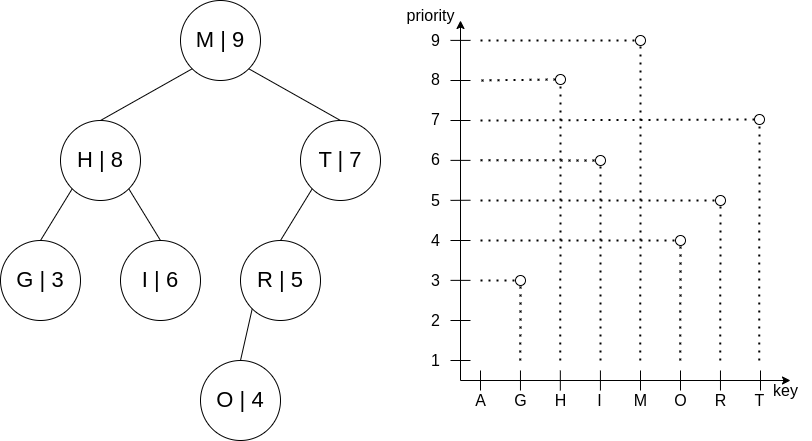
\includegraphics[width=300px]{images/4_Randomized_data_structures/cartesian_tree.png}
    \caption{Treap as cartesian partitioner}
\end{figure}

each point splits the plane in two different parts and each part is a sub-tree of the treap.
It's an efficient way to represent points for some kind of queries.

\subsection{Search for a letter}
It's a binary search tree for the letters so complexity is proportional to the height of the tree (NOT logarithmic): $O(h)$
    
\subsection{Find max/min priority}
Since the heap rules are observed we can do it in $O(h)$ too

\subsection{3-sided range query}
We want to find all the points in range $[a, b] \times [c, +\infty]$, so all points s.t.: $a \leq key \leq b$ and $c \leq priority$:
\begin{figure}[H]
    \centering
    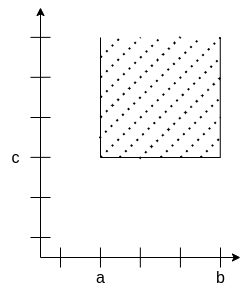
\includegraphics[width=150px]{images/4_Randomized_data_structures/three-sided-query.png}
    \caption{three-sided range query}
\end{figure}
being maximum heap for the priority when we go to a node we must check priority, if it's smaller than $c$ we can stop recursion, then being a BST when we are on a node if the key is outside the range $[a,b]$ we can stop branching in both children.
So we can execute a BFS and drop when the node doesn't match all requirements.

Ex: $[L, P] \times [5, +\infty]$
\begin{itemize}
    \item visit M|9: matches criteria so returns node;
    \item visit H|8: key outside range so exclude left tree;
    \item visit I|6: key outside range so exclude all tree since no children;
    \item visit T|7: key outside range so exclude right tree;
    \item visit R|5: key outside range so exclude right tree;
    \item visit O|4: key inside range but priority outside so totally stop recursion.
\end{itemize}

\subsubsection{Estimate cost}
Let's try to estimate the complexity: in the worst case we reach nodes in the limits of the ranges so all the nodes outside the path are dropped (maybe at first there is the check).
So in the worst case you check $O(h)$ nodes (two nodes for each node in the path) then for sure you visit all nodes inside the range until the priority is $ > c$.

So the cost is:
\begin{itemize}
    \item perculate the paths and drop lateral trees: $O(h)$;
    \item visit inside node until you don't exceed priority: $O(occurrences)$
\end{itemize}
in the end we have $O(h + occurrences)$.
The first part is not so ok since the treap can be very tall but we can balance it using rotations, the second part is optimal since is proportional to the answer to the query.

\subsection{Operations}
\subsubsection{Rotations}
To insert and delete elements we need \emph{rotations}:
\begin{figure}[H]
    \centering
    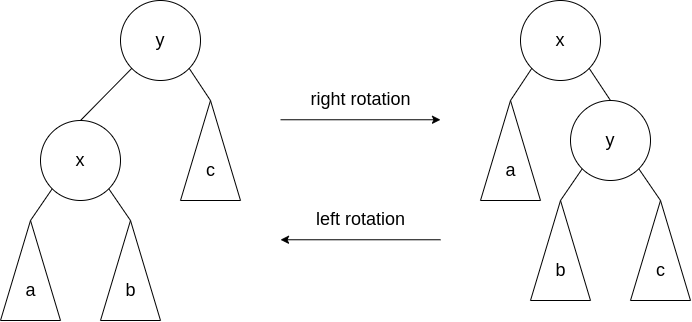
\includegraphics[width=300px]{images/4_Randomized_data_structures/treap_rotations.png}
    \caption{Rotations}
\end{figure}
We use right rotation when $priority(x) > priority(y)$ to promote $x$ and we use left rotation where $priority(y) > priority(x)$ to promote $y$.

\subsubsection{Insertion}
To insert an element we need to:
\begin{itemize}
    \item insert the new node respecting the key, as we would do in a BST;
    \item apply from the bottom to the top a series of rotation to comply with heap rules.
\end{itemize}

Ex: let's insert the node $(P,6)$:
\begin{figure}[H]
    \centering
    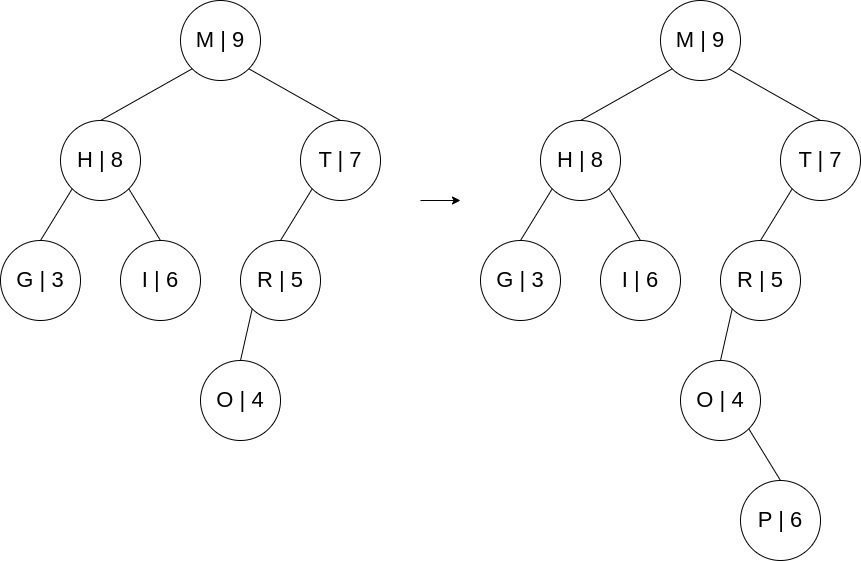
\includegraphics[width=300px]{images/4_Randomized_data_structures/insert_example_1.png}
    \caption{Insert the node respecting BST rules}
\end{figure}
we need to bubble up the node $(P,6)$ since it's priority is bigger than $(O,4)$:
\begin{figure}[H]
    \centering
    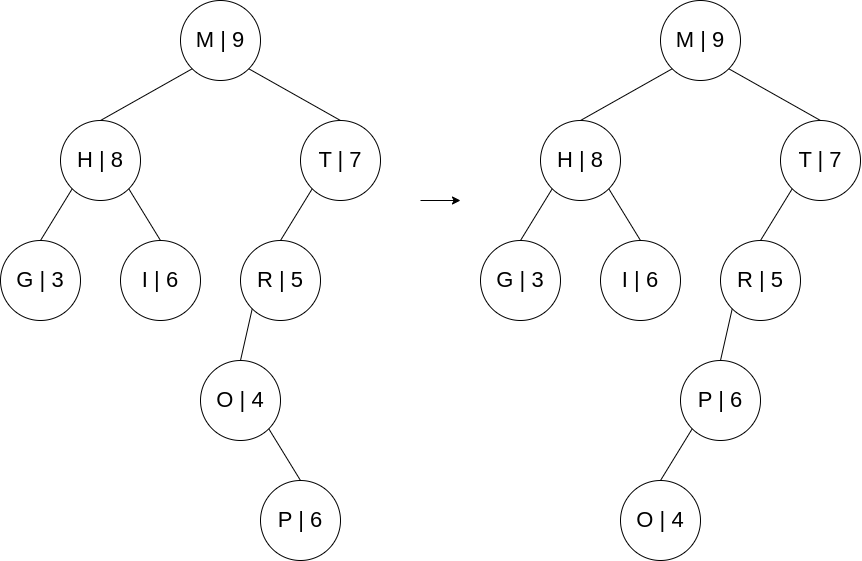
\includegraphics[width=300px]{images/4_Randomized_data_structures/insert_example_2.png}
    \caption{Left rotation}
\end{figure}
and now we need to bubble up that node again:
\begin{figure}[H]
    \centering
    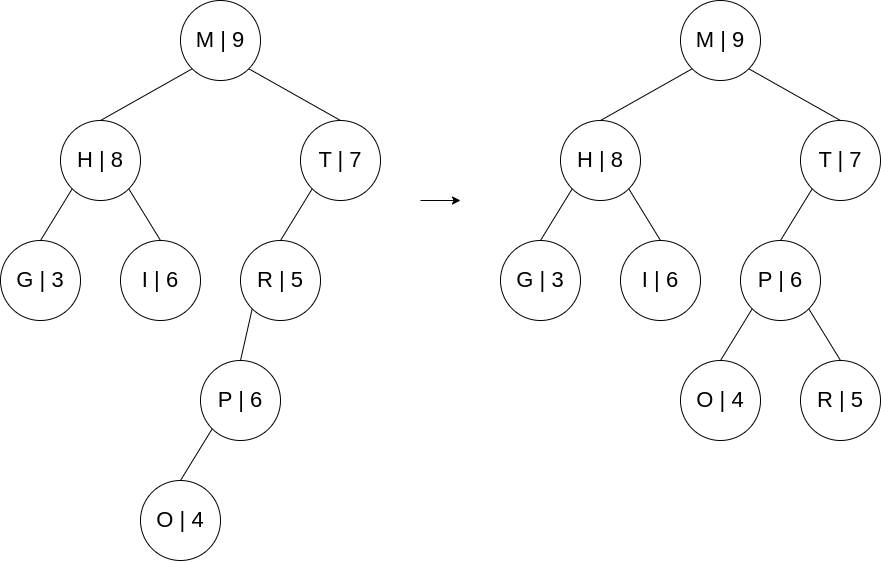
\includegraphics[width=300px]{images/4_Randomized_data_structures/insert_example_3.png}
    \caption{Right rotation}
\end{figure}

This operation is $O(h)$.

\subsubsection{Deletion}
To delete an element we exploit priority, as in heap:
\begin{itemize}
    \item we search for the key;
    \item we change the priority of that node to $-\infty$ (if using a max-heap, otherwise we use $+\infty$);
    \item we push that element down using rotations;
    \item once the element is a leaf we can safely delete it.
\end{itemize}

This operation is $O(h)$.

\subsubsection{Merge}
The $merge(T1, T2)$ operation allows us to join two different treap in a single one if and only if all keys in $T1 < $ all the keys in $T2$:
\begin{itemize}
    \item create a fake node with random key and priority $-\infty$ (if max-heap, otherwise $+\infty$);
    \begin{figure}[H]
        \centering
        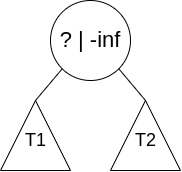
\includegraphics[width=100px]{images/4_Randomized_data_structures/merge.png}
        \caption{Fake node}
    \end{figure}
    \item push the fake root down;
    \item once the fake node is a leaf we can safely delete it.
\end{itemize}

\subsubsection{Split}
The $split(k)$ operations allows us to split a treap in two different ones in which the first one has only the keys $\leq k$ and the second one has only keys $> k$:
\begin{itemize}
    \item we insert a new node $(k, +\infty)$ (if max-heap, otherwise $-\infty$);
    \item we push the node up;
    \item once the node is the root we can delete the node and the two sons are the two new treaps;
\end{itemize}

\subsection{Treap as BST}
We can use the treap as a BST with random priority.
This is useful to obtain a balanced BST on average without too much overhead, moreover it also supports split and merge!

Let's prove that if the priorities are chosen at random then $h = (logn)$ on average: take $x_1, x_2, \_, x_n$ as the keys sorted for priority, then we define:
$$
A_k^i = 
\begin{cases}
    1 & \text{if $x_i$ is a proper ancestor of $x_k$ } \\
    0 & \text{otherwise}
\end{cases}
$$
then:
$$
    depth(X_k) = \sum_{i=1}^{n} A_k^i = \#\text{ancestors of } x_k
$$
we want to know on average what's the value:
$$
    \mathbb{E}[ depth(x_k) ] = \mathbb{E}\left[ \sum_{i=1}^n A_k^i \right] = \sum_{i=1}^n \mathbb{E}[A_k^i] = \sum_{i=1}^n \mathbb{P}(A_k^i = 1) 
$$
$x_i$ can be ancestor of $x_k$ only if $priority(x_k) > priority(x_i)$ so if $i < k$, we have 4 cases:
\begin{itemize}
    \item $x_i$ is root, it's a good case;
    \item $j < i$ and $x_j$ is root so both $x_i$ and $x_k$ are in the right sub-tree, we can't decide, we need to recurse;
    \item $j > i$ and $x_j$ is root so both $x_i$ and $x_k$ are in the left sub-tree, we can't decide, we need to recurse;
    \item $x_i \leq x_j \leq x_k$ and $j$ is root, surely $x_i$ is in the left sub-tree and $x_j$ is in the right sub-tree, so surely $x_i$ is not an ancestor of $x_k$.
\end{itemize}
We are left with a single case: $x_i, \_, x_j, \_, x_k$ whose probability is: $\frac{1}{|k - i| + 1}$ in which $|k - i|$ is the size of the subset $\{x_i, x_{i+1}, \_, x_k\}$, so in the end:
$$
    \sum_{i=1}^n \mathbb{P}(A_k^i = 1) = \sum_{i<k} \frac{1}{k-i+1} + \sum_{i>k} \frac{1}{i-k+1} \approx log_2 n
$$
since it's an harmonic sum.

\section{Skip list}
Skip list is widely used inside dictionaries, for example is a core part of redis: a key-value storage (a dictionary which implements insert, delete and search for a key).

We start from a list and keep the good insertion and deletion policy optimizing the search.
To improve search we create levels of list:
\begin{figure}[H]
    \centering
    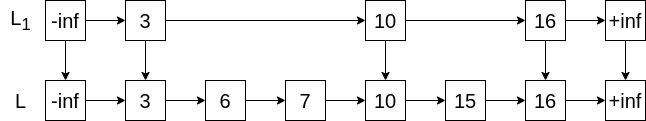
\includegraphics[width=250px]{images/4_Randomized_data_structures/deterministic_skip_list.png}
\end{figure}

If we would partition every $k$ elements each search would cost us:
$$
    k + \frac{n}{k}
$$
in which the first term is referred to the search in the $L_1$ and the second term is referred to the search in the $L_0$ partition.

The optimal choose of $k$ would be $k = \sqrt{n}$ but to keep that partition schema we should apply some algorithms during the insertion and deletion parts, we want to avoid to add that logic.
To avoid those shenanigans we randomize the data structure: during the construction of the overlay we toss a fair coin for each element in the list:
\begin{itemize}
    \item if we get tail: we copy the element from the list to the upper level;
    \item if we get head: we don't.
\end{itemize}
Using that algorithm we will build a newer level with $\approx \frac{n}{2}$ elements because the probability for each element of being chosen is $\frac{1}{2}$.
Of course nothing prevents us to iterate the process again and again until we get a level with a constant number of elements!

We will prove that to have a constant number of elements on a list we need $O(log_2 n)$ levels on high probability.

\subsection{Search}
To search for a key we start from $-\infty$ at the highest level and search like in all the lists. If we can't find the element we are looking for we stop at the first item greater than the key and start to search in the next level but in the the new range we get with the last element smaller than the key and the first element greater than it.
We go on with this approach until we find the key or until we reach the last list $+\infty$.

Example: searching for element 15:
\begin{figure}[H]
    \centering
    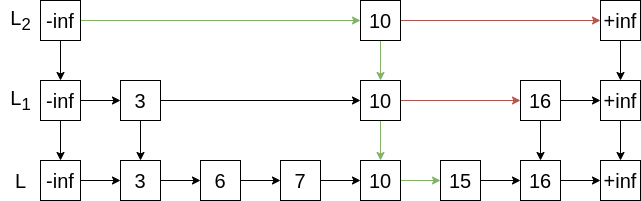
\includegraphics[width=250px]{images/4_Randomized_data_structures/skip_list_search.png}
\end{figure}
\begin{itemize}
    \item we start at $L_2$ and we check 10, we move on;
    \item we check for $+\infty$, since $10 < 15 < +\infty$ we go down from 10;
    \item we start at $L_1$ from 10 and we check 16, since $10 < 15 < 16$ we go down from 10;
    \item we start at $L$ from 10 and we check 15, we found a match ad we stop here returning the node.
\end{itemize}
Basically: go forth if next node is less than the target, otherwise go down.

The cost for search operation is $\#\text{horizontal pointers} + \#\text{vertical pointers}$ (the last one is the height of the structure, so the number of levels).

\subsection{Deletion}
We search for key, once we find it we delete the column associated with that element and connect the previous node with the next one, for each level in which the target element exists.

\subsection{Insertion}
First we find the position in which we should insert the element at the last level, then we insert the element in $L$ and we toss a coin to choose if we have to add the element in the upper level too.
NB: we insert the element after each last element checked for each level, we call that node \emph{the frontier}.

\subsection{Cost of search}
\subsubsection{Estimate the height}
Let's prove that with high probability the height is $O(log_2 n)$: first we define $L = \#$levels of skip list on $n$ items and we can say that:
$$
    L = max_k L(k)
$$
with $L(k)$ the level of the $k$-th item.
Then we can say that the probability for an item of having more than $l$ levels is:
$$
    \mathbb{P}(L(k) > l) = \left( \frac{1}{2} \right)^l
$$
which is the probability of having $l$ consecutive tails.
Moreover:
$$
    \mathbb{P}(L \geq l) = \mathbb{P}(max_k L(k) \geq l) = \mathbb{P}(\exists k : L(k) \geq l)
$$
we can use the so called \emph{union bound} to get an upper bound:
$$
    \mathbb{P}(\exists k : L(k) \geq l) \leq n \cdot \left( \frac{1}{2} \right)^l = \frac{n}{2^l}
$$
With this relation we can distinguish two cases:
\begin{itemize}
    \item $l \leq log_2 n \implies \frac{n}{2^l} \geq \frac{n}{2^{log_2 n}} = \frac{n}{n} = 1$: which is not so interesting as a case;
    \item $l > log_2 n \implies \frac{n}{2^l} < \frac{n}{2^{log_2 n}} = \frac{n}{n} = 1$: which is interesting since we want to know:
    $$
        \mathbb{P}(L \geq c \cdot log_2 n) \leq \frac{n}{2^{c \cdot log_2 n}} = \frac{n}{(2^{log_2 n})^c} = \frac{n}{n^c} = \frac{1}{n^{c-1}}
    $$
    and since $c \cdot log_2 n > log_2 n$ we are in this second case.
    That's the definition of \emph{with high probability}, so the probability of having more than a $c \cdot log_2 n$ levels, and so failing, is very small.
\end{itemize}

\subsubsection{Estimate the horizontal number of nodes in a search}
Take the path we perculate during a search and traverse it backwards, from bottom to top, we can notice:
\begin{itemize}
    \item starting from the bottom we can go to the left, so the node we are coming from in a normal search, until we find an upward pointer because once we find one we must go upward in the level.

    \item for each node the probability of having an upward pointer is $\frac{1}{2}$, since it depends on the result of a coin toss;
\end{itemize}
Since the average number of toss to get a tail is 2 we can say that on average we step 2 nodes horizontally for each level, so in total we have $2 \cdot log_2 n$ elements horizontally.

\subsubsection{Total cost}
So with high probability we have $O(log_2 n)$ vertical nodes and $O(log_2 n)$ horizontal nodes, in the end the search costs us $O(log_2 n)$.

NB: using this randomized data structure we achieve $O(log_2 n)$ search time avoiding the rotations we would have on a binary tree!

NB: skip list supports range queries too, so it's preferred to a dictionary in some contexts.